\documentclass[serif, xcolor=dvipsnames]{beamer}
\usepackage{bookman}
\usepackage[T1]{fontenc}
\usepackage[utf8]{inputenc}
\usepackage{textcomp}

\usepackage{graphicx}

%\usepackage{mathpazo}%Letra palatino con fuentes para matemáticas
\usepackage[T1]{fontenc}
\usepackage[utf8]{inputenc}
\usepackage{graphicx}
\usepackage{url}
\usepackage{amsmath}
\usepackage{booktabs}
\usepackage{textcomp}%%needed for the euro symbol

\date{}

\usepackage[emulate=units]{siunitx}
\sisetup{per=fraction, fraction=nice, decimalsymbol=comma}
\newunit{\wattpeak}{Wp}
\newunit{\watthour}{Wh}
\newunit{\amperehour}{Ah}

\setbeamercovered{transparent}
\setbeamertemplate{navigation symbols}{}
\usefonttheme{structuresmallcapsserif} 
\usefonttheme{serif} 
\usefonttheme{structurebold}

%\usepackage{epstopdf}


\usepackage[spanish]{babel}
\addto\shorthandsspanish{\spanishdeactivate{~<>}}

\hypersetup{pdfauthor={Oscar Perpi\~n\'an},%
    pdftitle={Energ\'ia Solar Fotovoltaica},%
    filecolor=blue,%
    urlcolor=blue}



%\usepackage{handoutWithNotes} %para hacer papel con notas 
%\pgfpagesuselayout{4 on 1 with notes}[a4paper,border shrink=5mm]



%\usepackage{pgfpages}
%\pgfpagesuselayout{2 on 1}[a4paper,border shrink=5mm]


%\usepackage{mathpazo}%Letra palatino con fuentes para matemáticas
\usepackage[T1]{fontenc}
\usepackage[utf8]{inputenc}
\usepackage{graphicx}
\usepackage{url}
\usepackage{amsmath}
\usepackage{booktabs}

\usepackage[spanish]{babel}
\addto\shorthandsspanish{\spanishdeactivate{~<>}}


\usepackage{hyperref}
% \hypersetup{pdfauthor={Oscar Perpi\~n\'an},%
%     pdftitle={Energ\'ia Solar Fotovoltaica},%
%     filecolor=blue,%
%     urlcolor=blue}

\hypersetup{
    bookmarks=true,         % show bookmarks bar?
%    unicode=true,          % non-Latin characters in Acrobat’s bookmarks
    bookmarksnumbered=false,
    bookmarksopen=false,
    breaklinks=true,
    backref=true,
    pdftoolbar=true,        % show Acrobat’s toolbar?
    pdfmenubar=true,        % show Acrobat’s menu?
    pdffitwindow=false,     % window fit to page when opened
    pdfstartview={FitH},    % fits the width of the page to the window
    pdftitle={Energía Solar Fotovoltaica},    % title
    pdfauthor={Oscar Perpiñán Lamigueiro},     % author
    pdfsubject={Electrotecnia},   % subject of the document
    pdfcreator={AucTeX/Emacs},   % creator of the document
    pdfproducer={LaTeX}, % producer of the document
    pdfnewwindow=true,      % links in new window
    pdfborder={0 0 0},
    colorlinks=true,       % false: boxed links; true: colored links
    linkcolor=,          % color of internal links
    citecolor=BrickRed,        % color of links to bibliography
    filecolor=black,      % color of file links
    urlcolor=Blue           % color of external links 
}

\usepackage[emulate=units]{siunitx}
\sisetup{per=fraction, fraction=nice, decimalsymbol=comma}
\newunit{\wattpeak}{Wp}
\newunit{\watthour}{Wh}
\newunit{\amperehour}{Ah}

\setbeamercovered{transparent}
\setbeamertemplate{navigation symbols}{}
\usefonttheme{serif} 
\usefonttheme{structuresmallcapsserif} 

\useinnertheme[shadow=true]{rounded}
\useoutertheme{shadow}
%\usecolortheme[named=BrickRed]{structure} %sirve para cambiar el color genérico
\usecolortheme{orchid}
\usecolortheme{whale}
\documentclass[xcolor={usenames,svgnames,dvipsnames}]{beamer}
\usepackage[utf8]{inputenc}
\usepackage[T1]{fontenc}
\usepackage{graphicx}
\usepackage{grffile}
\usepackage{longtable}
\usepackage{wrapfig}
\usepackage{rotating}
\usepackage[normalem]{ulem}
\usepackage{amsmath}
\usepackage{textcomp}
\usepackage{amssymb}
\usepackage{capt-of}
\usepackage{hyperref}
\usepackage{color}
\usepackage{listings}
\usepackage{mathpazo}
\usepackage{gensymb}
\usepackage{amsmath}
\usepackage{chemarr}%flechas para reacciones químicas (SFER.tex)
\bibliographystyle{plain}
\AtBeginSubsection[]{\begin{frame}[plain]\tableofcontents[currentsubsection,sectionstyle=show/shaded,subsectionstyle=show/shaded/hide]\end{frame}}
\AtBeginSection[]{\begin{frame}[plain]\tableofcontents[currentsection,hideallsubsections]\end{frame}}
\usepackage[emulate=units]{siunitx}
\sisetup{fraction=nice, decimalsymbol=comma, retain-unity-mantissa = false}
\newunit{\wattpeak}{Wp}
\newunit{\watthour}{Wh}
\newunit{\amperehour}{Ah}
\usepackage{steinmetz}
\hypersetup{colorlinks=true, linkcolor=OliveGreen, urlcolor=Blue}
\renewcommand{\thefootnote}{\fnsymbol{footnote}}
\beamertemplatenavigationsymbolsempty
\setbeamertemplate{footline}[frame number]

\setbeamercolor{alerted text}{fg=Green!50!black} \setbeamerfont{alerted text}{series=\bfseries}
\usefonttheme{serif}
\setbeamercovered{transparent}
\setbeamertemplate{navigation symbols}{}
\usefonttheme{serif} 

\setbeamercolor{palette primary}{bg=OliveGreen,fg=white}
\setbeamercolor{palette secondary}{bg=OliveGreen,fg=white}
\setbeamercolor{palette tertiary}{bg=OliveGreen,fg=white}
\setbeamercolor{palette quaternary}{bg=OliveGreen,fg=white}
\setbeamercolor{structure}{fg=OliveGreen} % itemize, enumerate, etc
\setbeamercolor{section in toc}{fg=OliveGreen} % TOC sections

\usetheme[hideothersubsections]{Goettingen}

\usepackage{tikz}

\titlegraphic{
\includegraphics[width=2.5cm]{../figs/logoEOI.jpg}}
\addtobeamertemplate{frametitle}{}{%
\begin{tikzpicture}[remember picture,overlay]
\node[anchor=south east,yshift=2pt] at (current page.south east) {
\includegraphics[width=1.5cm]{../figs/logoEOI.jpg}};
\end{tikzpicture}}



\usepackage[spanish]{babel}
\addto\shorthandsspanish{\spanishdeactivate{~<>}}

\begin{document}

\title{\textsc{Electrotecnia}}


\author{\textsc{Oscar Perpiñán Lamigueiro}}
\date{}

\frame[plain]{\titlepage}


\setcounter{tocdepth}{1}%Solo quiero que aparezcan las secciones
\AtBeginSection[]{
    \begin{frame}
        \frametitle{Índice}
        \tableofcontents[currentsection] 
    \end{frame} 

                  }

\selectlanguage{spanish}%


\begin{frame}[plain]
\frametitle{Índice}

\tableofcontents{}


\end{frame}
\section{Conceptos preliminares}

\subsection{Definiciones}

\begin{frame}
  \frametitle{Sistema de suministro eléctrico}

  Un \textbf{sistema de suministro eléctrico} tienen como objetivo
  \textbf{producir, transportar y distribuir energía eléctrica} a los
  lugares de consumo, con el mínimo coste posible en condiciones de
  \textbf{fiabilidad, calidad y seguridad}.

  Se pueden identificar diferentes componentes del sistema:
  \begin{itemize}
  \item Generadores
  \item Redes de transporte
  \item Redes de distribución
  \item Equipos de acondicionamiento, transformación y protección (y
    en algunos casos, almacenamiento)
  \item Puntos de consumo
  \end{itemize}

\end{frame}
\begin{frame}
  \frametitle{Sistema de suministro eléctrico}

  \begin{center}
    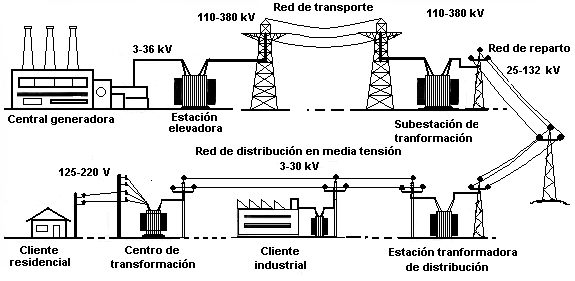
\includegraphics[scale=0.5]{../Figuras/Figuras_Externas/Redelectrica2}
    \par\end{center}


\end{frame}


\begin{frame}
  \frametitle{Electricidad}
  \begin{itemize}
  \item La electricidad es un fenómeno físico asociado al
    \textbf{movimiento de las cargas eléctricas}.
  \item El aprovechamiento de la electricidad consiste en generar y
    canalizar el movimiento de las cargas eléctricas.
  \item El movimiento de las cargas eléctricas es la \textbf{corriente
      eléctrica}.  Este movimiento se realiza mediante un trabajo,
    cuantificado por el \textbf{potencial}.
  \end{itemize}

\end{frame}
\begin{frame}
  \frametitle{Intensidad de Corriente eléctrica}
  \begin{itemize}
  \item \textbf{Variación de la carga con el tiempo en la sección
      transversal de un conductor}
    \[
    i(t)=\frac{dq(t)}{dt}
    \]

  \item Movimiento de electrones libres. Sin embargo, por convenio su
    sentido es positivo para el movimiento de las cargas positivas.
  \item \textbf{Principio de conservación de la carga}: las lineas de
    corriente son cerradas (o solenoidales)

    \begin{itemize}
    \item Primera ley de Kirchhoff : la suma de las corrientes que
      llegan a un nudo es igual a la suma de las que salen.
    \end{itemize}
  \end{itemize}

\end{frame}
\begin{frame}
  \frametitle{Tensión. Diferencia de potencial}
  \begin{itemize}
  \item \textbf{Trabajo realizado al mover una carga unidad entre dos
      puntos}.
  \end{itemize}
  \[
  v=\frac{dW_{e}}{dq}
  \]

  \begin{itemize}
  \item Si entre dos puntos A y B existe una diferencia de potencial,
    podemos escribir:
    \begin{eqnarray*}
      v_{AB} & = & v_{A}-v_{B}\\
      v_{AB} & = & -v_{BA}
    \end{eqnarray*}

  \end{itemize}

\end{frame}
\begin{frame}
  \frametitle{Potencia eléctrica}
  \begin{itemize}
  \item Trabajo realizado por unidad de tiempo
    \[
    p(t)=\frac{dW_{e}}{dt}=v(t)\cdot\frac{dq(t)}{dt}=v(t)\cdot i(t)
    \]

  \item Un elemento del circuito absorbe (\emph{receptor}) o entrega
    (\emph{generador}) potencia según el sentido de tensión y
    corriente en sus terminales
  \item \textbf{Principio de conservación de la energía}: la energía
    producida por un generador se consume por los receptores del
    circuito para producir trabajo (mecánico, químico, etc.) o calor.

    \begin{itemize}
    \item Segunda ley de Kirchhoff: la suma (con signo) de las
      tensiones a lo largo de un camino cerrado (circuito) es cero
    \end{itemize}
  \end{itemize}

\end{frame}
\begin{frame}
  \frametitle{Potencia eléctrica}
  \begin{description}
  \item [{Ejemplo:}] en el dipolo de la figura se absorbe potencia
    ($p(t)>0$)
  \end{description}
  \begin{center}
    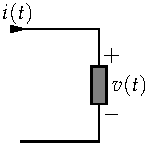
\includegraphics{../Figuras/ReceptorPasivo}
    \par\end{center}


\end{frame}
\begin{frame}
  \frametitle{Potencia y Energía}
  \begin{description}
  \item [{Energía}] es la capacidad para realizar un trabajo.


    Unidades Wh, kWh


    1 kWh = 3.6 MJ

  \item [{Potencia}] es la cantidad de trabajo efectuado \emph{por
      unidad de tiempo}.


    Unidades W, kW

  \end{description}

\end{frame}
\begin{frame}
  \frametitle{Eficiencia y Rendimiento}
  \begin{description}
  \item [{Eficiencia}] de un proceso es la relación entre la
    \emph{potencia} de salida y la \emph{potencia} de entrada a ese
    proceso.
  \item [{Rendimiento}] de un proceso es la relación entre la
    \emph{energía} de salida y la \emph{energía} de entrada a ese
    proceso.
  \end{description}

\end{frame}


\subsection{Elementos Lineales}


\begin{frame}
  \frametitle{Generadores}
  \begin{itemize}
  \item \textbf{Generador de tensión}: su tensión es independiente de
    la corriente (la corriente la fija el circuito)

    \begin{itemize}
    \item Batería electroquímica
    \item Inversor de electrificación rural a su salida
    \end{itemize}
  \end{itemize}
  \begin{center}
    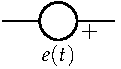
\includegraphics{../Figuras/GeneradorTension}
    \par\end{center}
  \begin{itemize}
  \item \textbf{Generador de corriente}: su corriente es independiente
    de la tensión (la tensión la fija el circuito)

    \begin{itemize}
    \item Inversor de conexión a red a su salida
    \end{itemize}
  \end{itemize}
  \begin{center}
    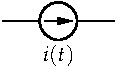
\includegraphics{../Figuras/GeneradorCorriente}
    \par\end{center}


\end{frame}
\begin{frame}
  \frametitle{Resistencia}
  \begin{itemize}
  \item \textbf{Produce una caída de tensión entre sus terminales
      directamente proporcional a la corriente que lo atraviesa}.
  \item La constante de proporcionalidad es el valor de la
    resistencia: $V=R\cdot I$
  \item Su valor depende de resistividad del material, de la sección y
    de la longitud: $R=\rho\cdot\frac{L}{S}$
  \item Disipa energía eléctrica produciendo \textbf{calor}:
    $p(t)=R\cdot i^{2}(t)$
  \item Cortocircuito: resistencia nula (tensión nula); Circuito
    abierto: resistencia infinita (corriente nula).
  \end{itemize}
  \begin{center}
    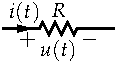
\includegraphics{../Figuras/Resistencia}
    \par\end{center}


\end{frame}
\begin{frame}
  \frametitle{Bobina o inductancia}
  \begin{itemize}
  \item Cuando una corriente oscilante atraviesa un conductor
    arrollado se produce una \textbf{tensión inducida que se opone a
      esta corriente} (ley de Faraday y Lenz)
  \item La constante que liga la tensión en sus terminales con el
    cambio de la corriente es el valor de la inductancia
    \[
    v(t)=L\cdot\frac{di(t)}{dt}
    \]

  \item Almacena \textbf{energía magnética}.
  \item La bobina \textbf{retrasa los cambios de la corriente}
    respecto de la tensión.
  \item En circuitos de corriente continua es un cortocircuito.
  \end{itemize}
  \begin{center}
    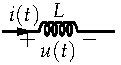
\includegraphics{../Figuras/Bobina}
    \par\end{center}


\end{frame}
\begin{frame}
  \frametitle{Condensador}
  \begin{itemize}
  \item Cuando se establece una tensión entre dos placas metálicas
    separadas por una capa dieléctrica, se produce una
    \textbf{separación de cargas que se acumulan en cada placa}, con
    signos contrarios.
  \item Almacena \textbf{energía eléctrica}
  \item La constante de proporcionalidad entre la carga acumulada y la
    tensión entre las placas es la capacidad
    \[
    C=\frac{Q}{V_{AB}}
    \]

  \end{itemize}
  \begin{center}
    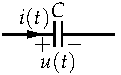
\includegraphics{../Figuras/Condensador}
    \par\end{center}


\end{frame}
\begin{frame}
  \frametitle{Condensador}
  \begin{itemize}
  \item En el proceso de carga\c{ }se produce una corriente eléctrica
    entre las dos placas
    \[
    i(t)=\frac{dq(t)}{d(t)}=C\frac{dv(t)}{dt}
    \]

  \item \textbf{Retrasa las variaciones de la tensión respecto de la
      corriente}
  \item En un circuito de corriente continua\c{ } cuando el
    condensador está cargado se comporta como un circuito abierto.
  \end{itemize}

\end{frame}

\subsection{Elementos No Lineales}

\begin{frame}
  \frametitle{Diodo}
  \begin{itemize}
  \item Un diodo es un dispositivo electrónico que permite el paso de
    corriente a través de él a partir de una tensión de polarización.
  \item Cuando no conduce se comporta (idealmente) como un circuito
    abierto.  Cuando conduce se comporta (idealmente) como un
    cortocircuito.
  \item Por tanto, puede ser utilizado como

    \begin{itemize}
    \item \textbf{Elemento de bloqueo} (evitar que circule corriente
      por una parte del circuito en ciertas condiciones)
    \item \textbf{Elemento de protección} (obligar a que la corriente
      circule por él, evitando que circule por otra rama paralela).
    \end{itemize}
  \end{itemize}
  \begin{center}
    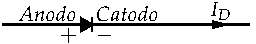
\includegraphics{../Figuras/Diodo}
    \par\end{center}


\end{frame}
\begin{frame}[plain]
  \frametitle{Transistor}
  \begin{itemize}
  \item Un transistor es un dispositivo electrónico con tres
    terminales que permite el paso de corriente entre dos de sus
    terminales cuando en el tercer terminal está polarizado
    adecuadamente.
  \item Cuando no conduce se comporta (idealmente) como un circuito
    abierto.  Cuando conduce se comporta (idealmente) como un
    cortocircuito.
  \end{itemize}
  Por tanto, puede ser utilizado como:
  \begin{columns}%{}


    \column{8cm}
    \begin{itemize}
    \item \textbf{Elemento de conmutación} (dirigir la circulación de
      corriente entre dos terminales controlando la señal en el tercer
      terminal)
    \item \textbf{Elemento de amplificación} (la señal entregada en el
      terminal de control es reproducida en la salida con mayor
      amplitud)
    \end{itemize}

    \column{3cm}


    \begin{center}
      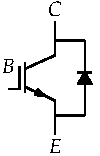
\includegraphics{../Figuras/Transistor}
      \par\end{center}

  \end{columns}%{}

\end{frame}

\subsection{Asociación de elementos pasivos}


\begin{frame}
  \frametitle{Conexión en serie }


  \framesubtitle{Misma corriente por todos los elementos: la tensión
    se reparte}
  \begin{columns}[c]%{}


    \column{3cm}


    $R_{s}=\sum_{i}R_{i}$


    $L_{s}=\sum_{i}L_{i}$


    $\frac{1}{C_{s}}=\sum_{i}\frac{1}{C_{i}}$


    \column{5cm}


    \begin{center}
      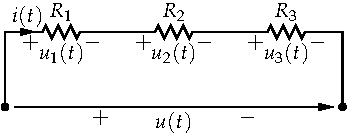
\includegraphics{../Figuras/AsociacionSerie}
      \par\end{center}

  \end{columns}%{}

\end{frame}
\begin{frame}
  \frametitle{Conexión en paralelo}


  \framesubtitle{Misma tensión aplicada a todos los elementos: la
    corriente se reparte}
  \begin{columns}[c]%{}


    \column{3cm}


    $\frac{1}{R_{p}}=\sum_{i}\frac{1}{R_{i}}$


    $\frac{1}{L_{p}}=\sum_{i}\frac{1}{L_{i}}$


    $C_{p}=\sum_{i}C_{i}$


    \column{5cm}


    \begin{center}
      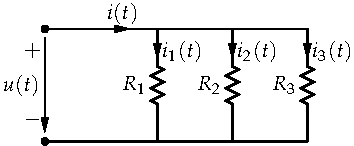
\includegraphics{../Figuras/AsociacionParalelo}
      \par\end{center}

  \end{columns}%{}

\end{frame}



\section{Corriente alterna sinusoidal}


\subsection{Conceptos Fundamentales}

\begin{frame}
  \frametitle{Pulsación - Frecuencia - Fase}

\[
y(t)=Y_{m}\cdot\cos(\omega\cdot t+\varphi)
\]

\begin{itemize}
\item T: periodo de la onda (segundos)
\item $\omega=\frac{2\cdot\pi}{T}$: pulsación (radianes/segundo)
\item $f=\frac{\omega}{2\cdot\pi}=\frac{1}{T}$: frecuencia (Hz)
\item $\varphi$: fase (radianes o grados)

  \begin{itemize}
  \item Es el argumento de la onda para t=0
  \item Tomando una onda como referencia, si la fase es 0º, se dice
    que están en fase con la onda de referencia.
  \item Ídem, si la fase es 90º, se dice que están en cuadratura.
  \item Ídem, si la fase es positiva, se dice que la onda adelanta
    respecto a la referencia.
  \end{itemize}
\item $Y_{m}$ valor máximo de la onda.
\end{itemize}

\end{frame}
\begin{frame}[plain]
  \frametitle{Pulsación - Frecuencia - Fase}

\[
y(t)=Y_{m}\cdot\cos(\omega\cdot t+\varphi)
\]


\begin{center}
  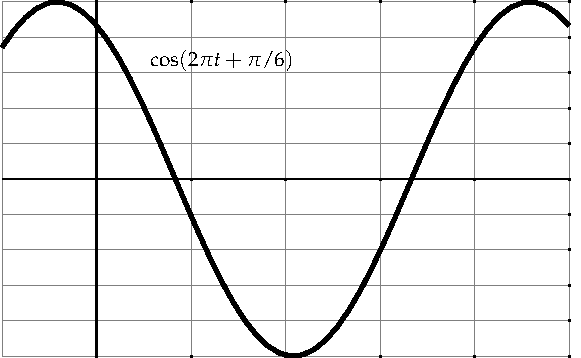
\includegraphics{../Figuras/Sin}
  \par\end{center}


\end{frame}
\begin{frame}
  \frametitle{Valor medio y valor eficaz}
  \begin{itemize}
  \item \textbf{Valor medio}:
    \[
    \overline{Y}=\frac{1}{T}\int_{0}^{T}y(t)
    \]


    \begin{itemize}
    \item Para señal sinusoidal:
      \[
      \overline{Y}=\frac{1}{T}\int_{0}^{T}Y_{m}\cdot\cos(\omega\cdot
      t+\phi)\, dt=0
      \]

    \end{itemize}
  \item \textbf{Valor eficaz}:
    \[
    Y=\sqrt{\overline{y^{2}(t)}}=\sqrt{\frac{1}{T}\cdot\int_{0}^{T}y^{2}(t)}
    \]


    \begin{itemize}
    \item Para señal sinusoidal:
    \end{itemize}
  \end{itemize}
  \[
  Y=\sqrt{\frac{1}{T}\cdot\int_{0}^{T}\left(Y_{m}\cdot\cos(\omega\cdot
      t+\phi)\right)^{2}dt}=\frac{Y_{m}}{\sqrt{2}}
  \]



\end{frame}
\begin{frame}
  \frametitle{Representación fasorial}

\[
\vec{Y}=Y\cdot e^{j\phi}=Y\cdot(\cos(\phi)+\mathrm{j}\cdot\sin(\phi))
\]


\begin{center}
  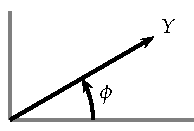
\includegraphics{../Figuras/Fasor}
  \par\end{center}


\end{frame}
\subsection{Impedancia}

\begin{frame}
  \frametitle{Impedancia}

\begin{eqnarray*}
  \vec{R} & = & R\\
  \vec{X_{c}} & = & \frac{1}{j\omega C}\\
  \vec{X_{L}} & = & j\omega L
\end{eqnarray*}


\begin{eqnarray*}
  \vec{Z} & = & R+jX\\
  \vec{Z} & = & Z\cdot e^{j\phi_{Z}}\\
  Z & = & \sqrt{R^{2}+X^{2}}\\
  \tan(\phi_{Z}) & = & \frac{X}{R}
\end{eqnarray*}



\end{frame}
\begin{frame}
  \frametitle{Impedancia}

\[
\vec{I}=\frac{\vec{V}}{\vec{Z}}=\frac{V}{Z}\cdot
e^{j(\phi_{V}-\phi_{Z})}=I\cdot e^{j\phi_{I}}
\]


\begin{center}
  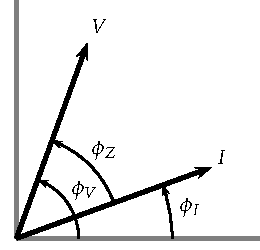
\includegraphics{../Figuras/Impedancia}
  \par\end{center}


\end{frame}
\begin{frame}
  \frametitle{Convenio de signos para Desfase}
  \begin{itemize}
  \item La tensión es origen de fases ($\phi_{V}=0$).
  \item La corriente está retrasada de la tensión un ángulo $\phi$
    positivo:
    \begin{eqnarray*}
      \phi_{I} & = & -\phi=\phi_{V}-\phi_{Z}\\
      \phi & = & \phi_{z}\\
      i(t) & = & I_{m}\cdot\cos(\omega\cdot t-\phi)
    \end{eqnarray*}

  \item Por tanto, \textbf{si el circuito es inductivo (retrasa fase
      de corriente respecto de tensión) $\phi$ es positivo}.
  \end{itemize}

\end{frame}
\begin{frame}[plain]
  \frametitle{Circuito Capacitivo puro}

  \begin{center}
    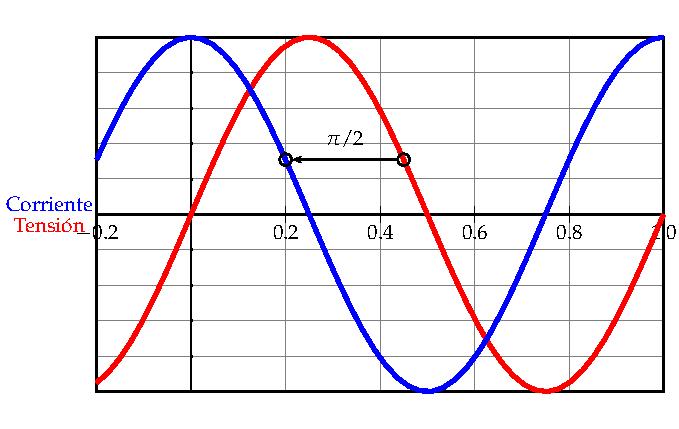
\includegraphics{../Figuras/PlotCircuitoCapacitivoPuro}
    \par\end{center}


\end{frame}
\begin{frame}[plain]
  \frametitle{Circuito Inductivo puro}

  \begin{center}
    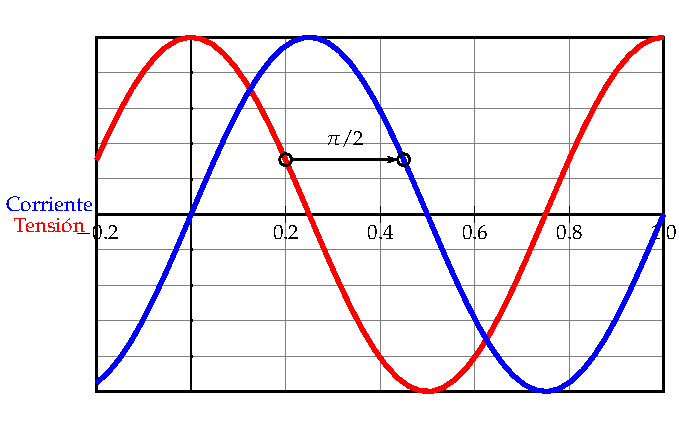
\includegraphics{../Figuras/PlotCircuitoInductivoPuro}
    \par\end{center}


\end{frame}
\begin{frame}[plain]
  \frametitle{Circuito Capacitivo}

  \begin{center}
    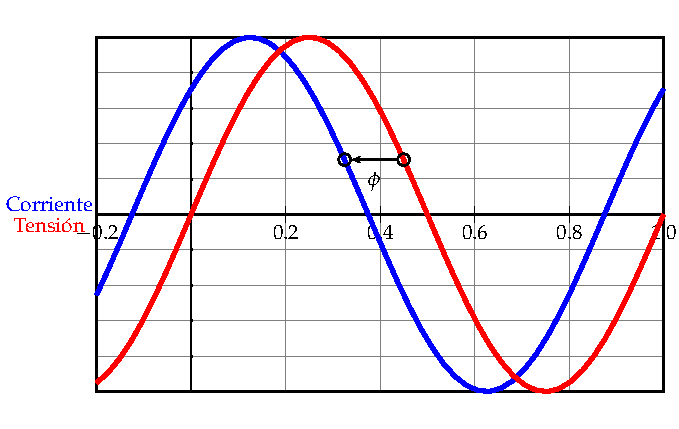
\includegraphics{../Figuras/PlotCircuitoCapacitivo}
    \par\end{center}


\end{frame}
\begin{frame}[plain]
  \frametitle{Circuito Inductivo}

  \begin{center}
    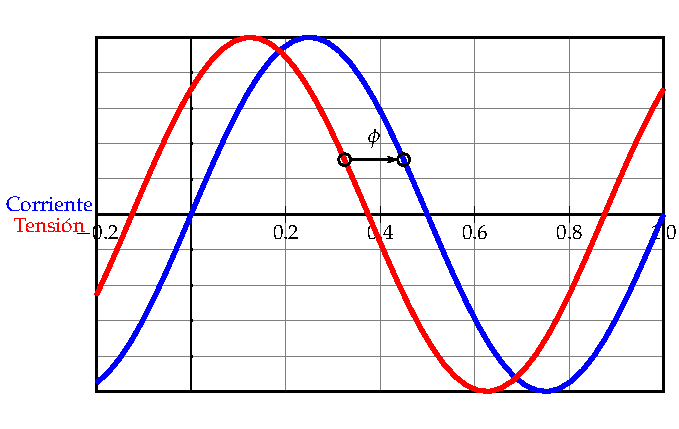
\includegraphics{../Figuras/PlotCircuitoInductivo}
    \par\end{center}


\end{frame}
\subsection{Potencia}


\begin{frame}[plain]
  \frametitle{Circuito Capacitivo puro}


  \framesubtitle{Potencia}

  \begin{center}
    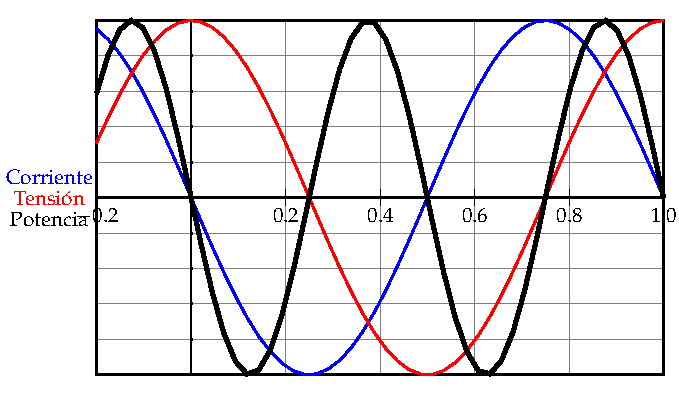
\includegraphics{../Figuras/PlotCircuitoCapacitivoPuro_Potencia}
    \par\end{center}


\end{frame}
\begin{frame}[plain]
  \frametitle{Circuito Inductivo puro}


  \framesubtitle{Potencia}

  \begin{center}
    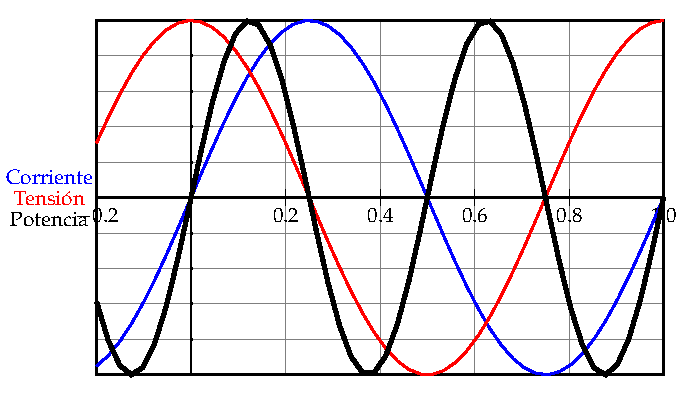
\includegraphics{../Figuras/PlotCircuitoInductivoPuro_Potencia}
    \par\end{center}


\end{frame}
\begin{frame}[plain]
  \frametitle{Circuito Capacitivo}


  \framesubtitle{Potencia}

  \begin{center}
    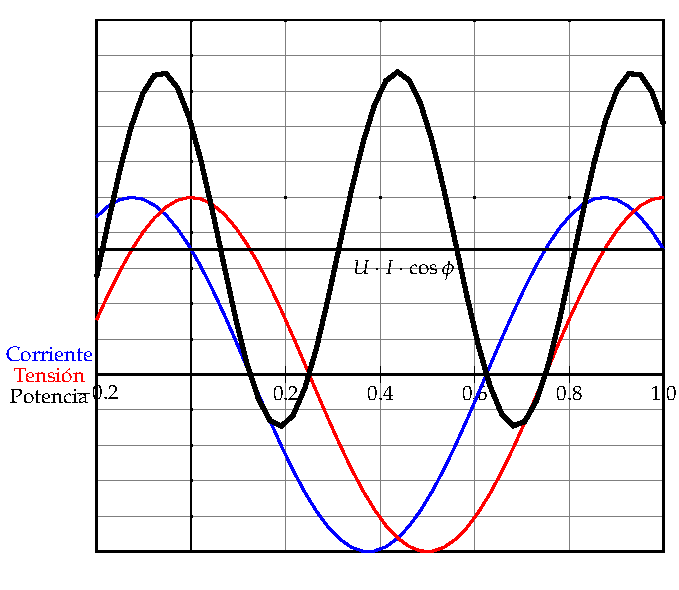
\includegraphics[scale=0.8]{../Figuras/PlotCircuitoCapacitivo_Potencia}
    \par\end{center}


\end{frame}
\begin{frame}[plain]
  \frametitle{Circuito Inductivo}


  \framesubtitle{Potencia}

  \begin{center}
    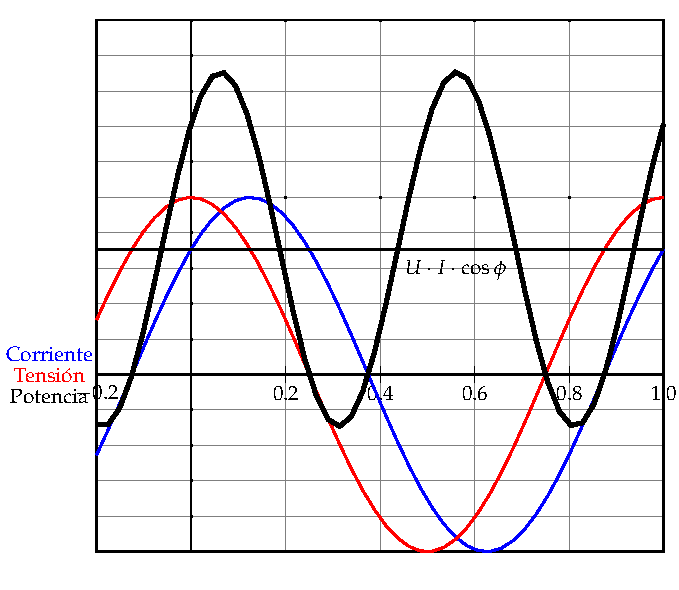
\includegraphics[scale=0.8]{../Figuras/PlotCircuitoInductivo_Potencia}
    \par\end{center}


\end{frame}
\begin{frame}
  \frametitle{Potencia Activa, Reactiva y Aparente}

\begin{eqnarray*}
  P & = & V\cdot I\cdot\cos(\phi)\\
  Q & = & V\cdot I\cdot\sin(\phi)\\
  S & = & P+jQ
\end{eqnarray*}



\end{frame}
\begin{frame}
  \frametitle{Potencia de elementos}
  \begin{itemize}
  \item Una \textbf{resistencia sólo consume potencia activa}
    ($\cos(\phi)=1$).
  \item Un \textbf{condensador no consume potencia activa}
    ($\cos(\phi)=0$), y \textbf{entrega potencia reactiva}
    ($\sin(\phi)=-1$)
  \item Una \textbf{bobina no consume potencia activa}
    ($\cos(\phi)=0$) y \textbf{absorbe potencia reactiva}
    ($\sin(\phi)=1$)
  \end{itemize}

\end{frame}
\begin{frame}
  \frametitle{Compensación de reactiva}
  \begin{itemize}
  \item El factor de potencia ($\cos(\phi)$) representa el desfase
    entre tensión y corriente.
  \item Es la fracción de potencia activa dentro de la potencia
    aparente.
  \item Suponiendo tensión constante, la corriente que debe circular
    es $I=\frac{S}{V}=\frac{P}{V\cdot\cos(\phi)}$.
  \item Para alimentar una potencia activa determinada, \textbf{la
      corriente es tanto más alta cuanto menor el factor de potencia}.
  \item \textbf{Factores de potencia bajos} obligan a

    \begin{itemize}
    \item Utilizar \textbf{grandes secciones} de cable para
      transportar la misma potencia activa
    \item Generar \textbf{mayor potencia aparente} para alimentar la
      misma potencia activa
    \end{itemize}
  \end{itemize}

\end{frame}
\begin{frame}
  \frametitle{Compensación de reactiva}
  \begin{itemize}
  \item Comúnmente, el factor de potencia es \textbf{inductivo}
    (máquinas eléctricas industriales).
  \item La red debe suministrar potencia reactiva inductiva (problemas
    derivados de bajo factor de potencia)
  \item Es necesario alterar localmente el factor de potencia:

    \begin{itemize}
    \item Solución común: utilizar \textbf{bancos de condensadores}
      como suministradores de potencia reactiva.
    \end{itemize}
  \end{itemize}

\end{frame}
\begin{frame}
  \frametitle{Resonancia}

  Para un circuito serie R-L-C:

\[
Z=\sqrt{R^{2}+\left(\omega L-\frac{1}{\omega C}\right)^{2}}
\]


Si $\omega L=\frac{1}{\omega C}$ el circuito tiene carácter resistivo
(Z=R).

\[
f_{r}=\frac{1}{2\pi\sqrt{LC}}
\]


y por tanto el $\cos(\phi)=1$ (la potencia aparente coincide con la
activa).


\end{frame}
\subsection{Trifásica}

\begin{frame}
  \frametitle{Motivación de los sistemas trifásicos}
  \begin{itemize}
  \item La potencia instantánea de un sistema monofásico es
    pulsante. En un sistema trifásico la potencia instantánea es
    constante, evitando vibraciones y esfuerzos en las máquinas.
  \item Para transportar una determinada potencia la masa de conductor
    necesaria es un 25\% en un trifásico que en un monofásico.
  \end{itemize}

\end{frame}
\begin{frame}[plain]
  \frametitle{Generación de un sistema trifásico}

  \begin{center}
    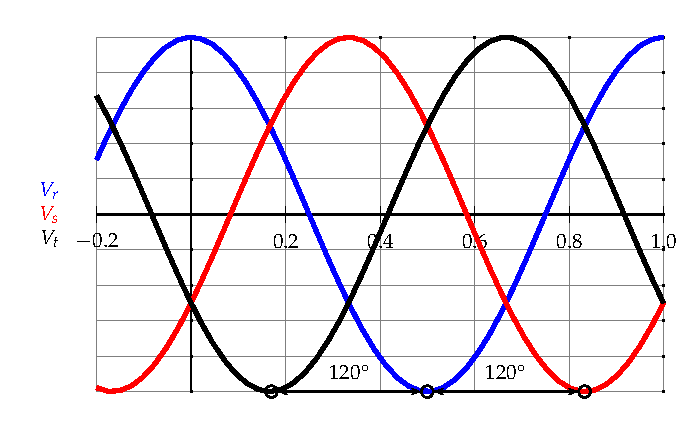
\includegraphics{../Figuras/TensionesTrifasica}
    \par\end{center}


\end{frame}
\begin{frame}[plain]
  \frametitle{Fase y línea}


  \framesubtitle{Receptor en Estrella (cuatro hilos, 3F+1N)}
  \begin{block} {}

    \begin{center}
      \[
      V_{L}=\sqrt{3}\cdot V_{F}
      \]
      \[
      I_{F}=I_{L}
      \]
      \[
      P=3\cdot V_{F}I_{F}\cos(\phi)=\sqrt{3}V_{L}I_{L}\cos(\phi)
      \]
      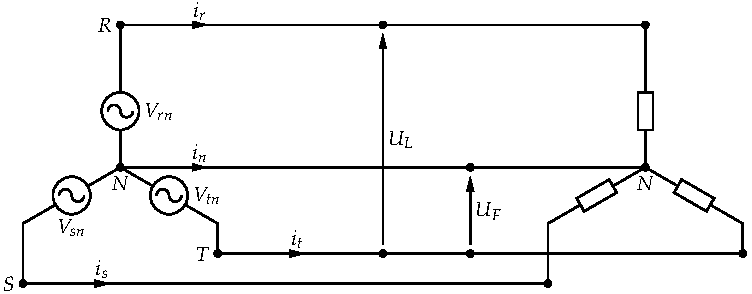
\includegraphics[scale=0.75]{../Figuras/RedTrifasicaEstrella}
      \par\end{center}

  \end{block}

\end{frame}
\begin{frame}[plain]
  \frametitle{Fase y línea}


  \framesubtitle{Receptor en Estrella (cuatro hilos, 3F+1N)}
  \begin{block} {}

    \begin{center}
      \[
      V_{L}=\sqrt{3}\cdot V_{F}
      \]
      \[
      I_{F}=I_{L}
      \]
      \[
      P=3\cdot V_{F}I_{F}\cos(\phi)=\sqrt{3}V_{L}I_{L}\cos(\phi)
      \]
      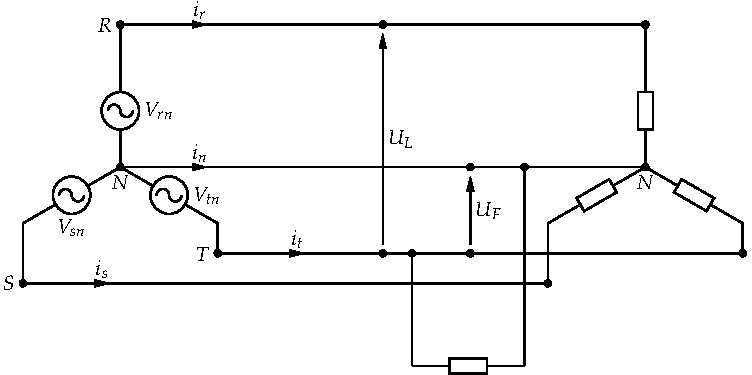
\includegraphics[scale=0.75]{../Figuras/RedTrifasicaEstrella_CargaMonofasica}
      \par\end{center}

  \end{block}

\end{frame}
\begin{frame}[plain]
  \frametitle{Fase y línea}


  \framesubtitle{Receptor en Triangulo (tres hilos, 3F)}
  \begin{block} {}

    \begin{center}
      \[
      V_{L}=V_{F}
      \]
      \[
      I_{F}=\frac{I_{L}}{\sqrt{3}}
      \]
      \[
      P=3\cdot V_{F}\cdot I_{F}\cos(\phi)=\sqrt{3}V_{L}I_{L}\cos(\phi)
      \]
      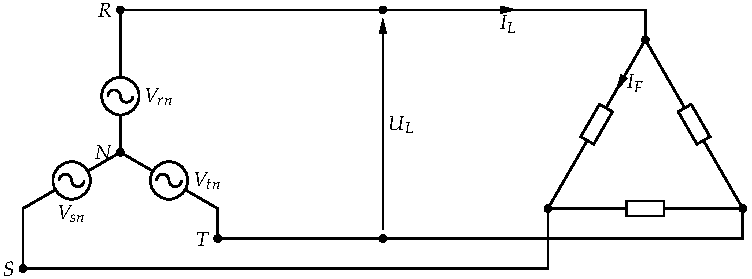
\includegraphics[scale=0.75]{../Figuras/RedTrifasicaEstrella_CargaTriangulo}
      \par\end{center}

  \end{block}

\end{frame}
\begin{frame}[plain]
  \frametitle{Fase y línea}


  \framesubtitle{Receptor en Triangulo (tres hilos, 3F)}
  \begin{block} {}

    \begin{center}
      \[
      V_{L}=V_{F}
      \]
      \[
      I_{F}=\frac{I_{L}}{\sqrt{3}}
      \]
      \[
      P=3\cdot V_{F}\cdot I_{F}\cos(\phi)=\sqrt{3}V_{L}I_{L}\cos(\phi)
      \]
      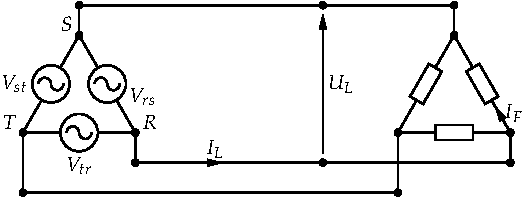
\includegraphics{../Figuras/RedTrifasicaTriangulo}
      \par\end{center}

  \end{block}

\end{frame}

\section{Máquinas Eléctricas}

\subsection{Fundamentos de Electromagnetismo}



\begin{frame}
  \frametitle{Electromagnetismo}
  \begin{itemize}
  \item Un campo magnético ejerce una fuerza sobre una carga en
    movimiento.  (Fuerza de Lorentz)
  \end{itemize}
  \begin{center}
    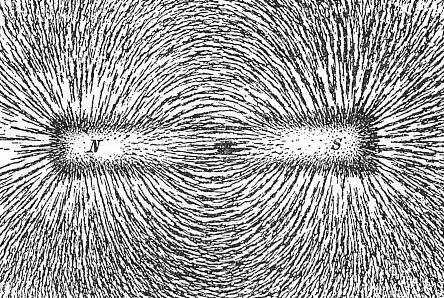
\includegraphics[scale=0.5]{../Figuras/Figuras_Externas/Magnet0873}
    \par\end{center}


\end{frame}
\begin{frame}
  \frametitle{Electromagnetismo}
  \begin{itemize}
  \item Una corriente eléctrica crea un campo magnético en torno al
    conductor.  (Oersted, Biot-Savart)
  \end{itemize}
  \begin{center}
    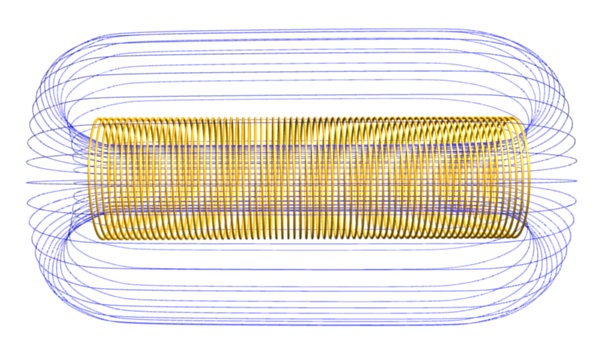
\includegraphics[scale=0.45]{../Figuras/Figuras_Externas/Solenoide}
    \par\end{center}


\end{frame}
\begin{frame}
  \frametitle{Electromagnetismo}
  \begin{itemize}
  \item Un conductor por el que circula corriente, situado en el seno
    de un campo magnético, altera este campo magnético, y experimenta
    una fuerza que lo expulsa para disminuir la alteración (Fuerza de
    Ampere)
  \end{itemize}
  \begin{center}
    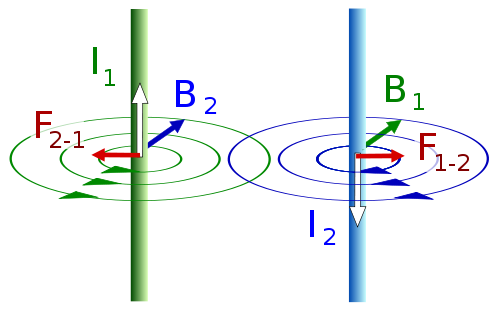
\includegraphics[scale=0.3]{../Figuras/Figuras_Externas/FuerzasRepulsion}
    \par\end{center}
  \begin{block} {}
    \centering Video:
    \href{http://www.youtube.com/watch?v=2j8D_N1v0tU}{Repulsión entre
      barras de Alta Tensión}
  \end{block}

\end{frame}
\begin{frame}
  \frametitle{Electromagnetismo}
  \begin{itemize}
  \item Entre los puntos extremos de una espira estática atravesada
    por un campo magnético, aparece una \textbf{tensión inducida
      siempre que el flujo magnético sea variable}. (Ley de Faraday).
  \item Esta condición se cumple cuando la \textbf{espira está en
      movimiento,} cuando el \textbf{campo magnético es variable}, o
    cuando ambas situaciones coinciden.
  \end{itemize}

\end{frame}
\begin{frame}
  \frametitle{Electromagnetismo}
  \begin{itemize}
  \item La tensión inducida es directamente proporcional a la rapidez
    con que cambia en el tiempo el flujo magnético que atraviesa la
    superficie encerrada por la espira.
    \[
    e=-\frac{\mathrm{d}\phi}{\mathrm{d}t}
    \]

  \item Al elemento que emite el campo magnético se le
    denomina\textbf{ inductor} y aquel que es atravesado por este
    flujo es el \textbf{inducido}.
  \end{itemize}

\end{frame}
\begin{frame}[plain]
  \frametitle{Electromagnetismo}

  \begin{center}
    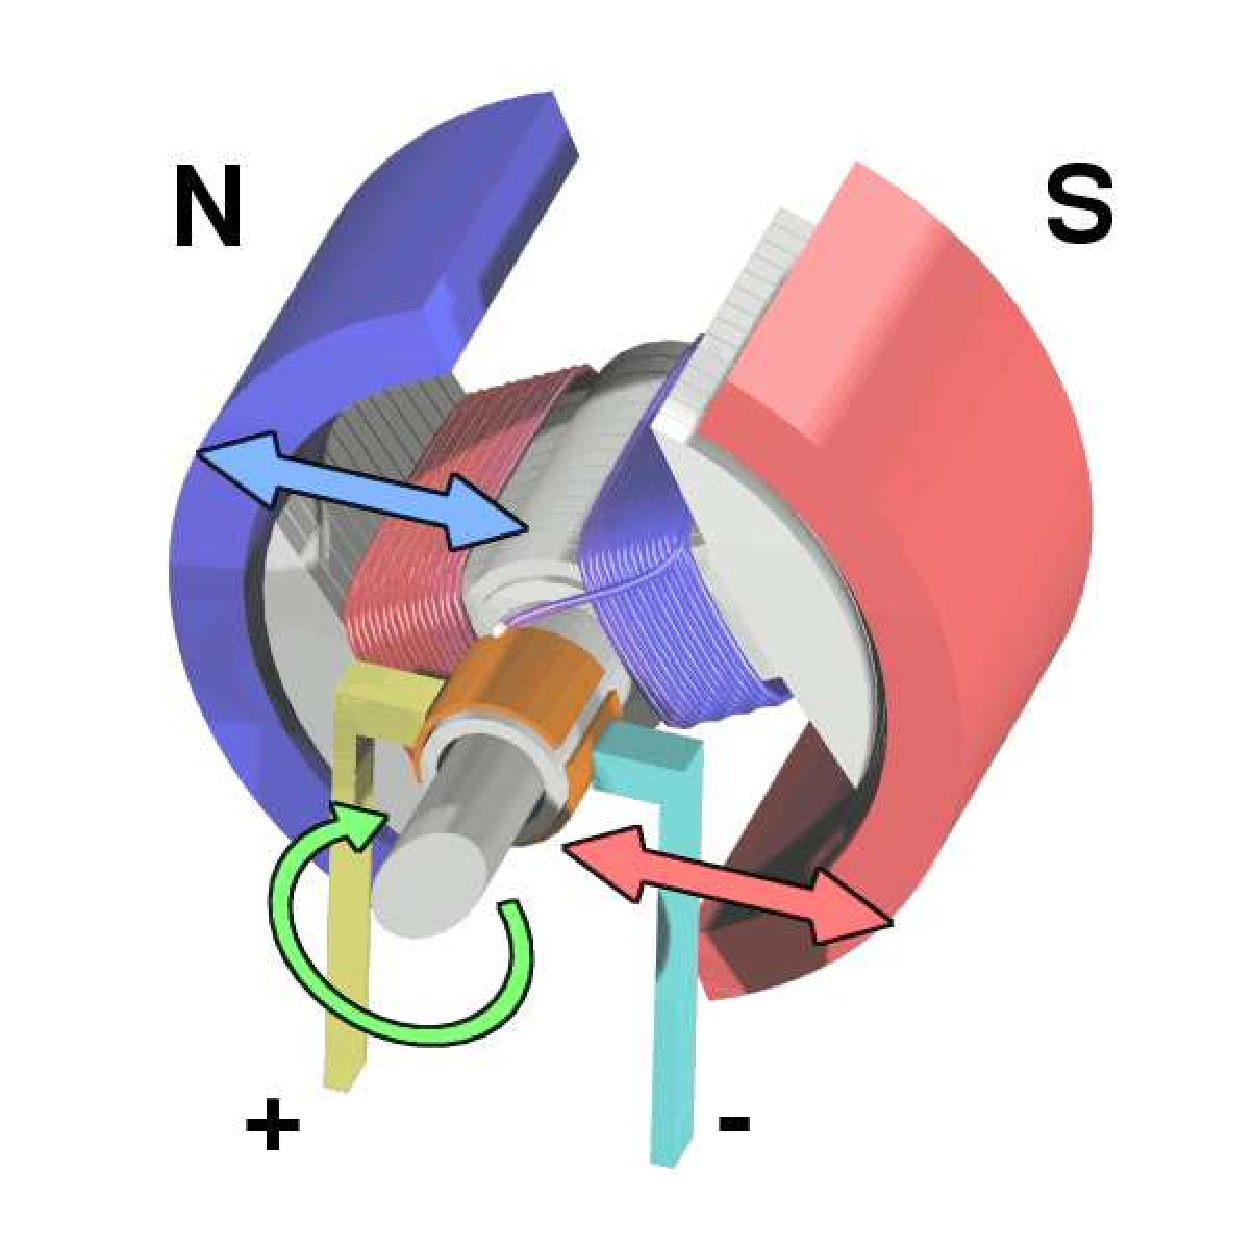
\includegraphics[scale=0.4]{../Figuras/Figuras_Externas/Electric_motor_cycle_3}
    \par\end{center}


\end{frame}
\begin{frame}
  \frametitle{Electromagnetismo}
  \begin{block} {Tensión, frecuencia y flujo}

\begin{eqnarray*}
  E & = & 4.44\cdot N\cdot\phi\cdot f
\end{eqnarray*}

\begin{itemize}
\item $E$ es la tensión inducida; $N$ número de espiras; $\phi$ es el
  flujo interceptado; $f$ frecuencia eléctrica
\item El flujo depende proporcionalmente de la tensión e inversamente
  de la frecuencia.
\end{itemize}
\end{block}

\end{frame}
\begin{frame}
  \frametitle{Electromagnetismo}
  \begin{block} {Par, potencia y velocidad}

\begin{eqnarray*}
  P & = & T\cdot\omega
\end{eqnarray*}

\begin{itemize}
\item $P$ es potencia mecánica; $T$ par mecánico; $\omega$ es la
  velocidad angular.
\item El par busca alinear los ejes magnéticos de inductor e inducido,
  o de estator y rotor. Una vez que están alineados, el par es nulo.
\end{itemize}
\end{block}

\end{frame}
\subsection{Tipos de máquinas}


\begin{frame}
  \frametitle{Relación de Frecuencias}
  \begin{block} {Frecuencia eléctrica y velocidad}

\begin{eqnarray*}
  f_{2} & = & f_{1}-n\cdot p
\end{eqnarray*}

\begin{itemize}
\item $f_{2}$ es la frecuencia en el inducido; $f_{1}$ es la
  frecuencia en el inductor; $n$ es la velocidad angular; $p$ es el
  número de polos.
\item Al utilizar colector de delgas (escobillas) en el inducido, la
  frecuencia en el circuito exterior ($f_{L}$) es diferente a $f_{2}$.
\end{itemize}
\end{block}

\end{frame}
\begin{frame}
  \frametitle{Clasificación de máquinas}
  \begin{itemize}
  \item Estáticas ($n=0\Rightarrow f_{2}=f_{1}$): Transformadores
  \item Rotativas ($n\neq0$):

    \begin{itemize}
    \item Flujo inductor constante ($f_{1}=0\Rightarrow f_{2}=n\cdot
      p$)

      \begin{itemize}
      \item Delgas ($f_{L}\neq f_{2}$): Máquinas de corriente continua
      \item Anillos ($f_{L}=f_{2}$): Máquinas síncronas
      \end{itemize}
    \item Flujo inductor variable ($f_{1}>0\Rightarrow
      f_{2}=f_{1}-n\cdot p$)

      \begin{itemize}
      \item Delgas ($f_{L}\neq f_{2}$): Motor universal
      \item Anillos ($f_{L}=f_{2}$): Máquinas asíncronas
      \end{itemize}
    \end{itemize}
  \end{itemize}

\end{frame}
\begin{frame}
  \frametitle{Transformador}
  \begin{itemize}
  \item Un transformador consiste en dos bobinas acopladas
    magnéticamente.
  \item Un transformador ideal tiene las siguientes relaciones entre
    tensión y corriente de entrada (primario) y salida
    (secundario):\end{itemize}
  \begin{columns}[c]%{}


    \column{3cm}


\[
N_{s}\cdot I_{s}=N_{p}\cdot I_{p}
\]
\[
\frac{V_{p}}{N_{p}}=\frac{V_{s}}{N_{s}}
\]



\column{5cm}


\begin{center}
  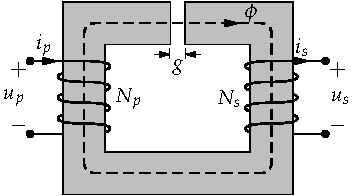
\includegraphics[scale=0.9]{../Figuras/Transformador2}
  \par\end{center}


\end{columns}%{}

\end{frame}
\begin{frame}
  \frametitle{Transformador}
  \begin{itemize}
  \item Un transformador ideal con relación de transformación
    $N_{p}/N_{s}<1$ (más vueltas en el secundario que en el primario),
    sube tensión ($V_{s}>V_{p}$) y reduce corriente ($I_{s}<I_{p}$).
  \end{itemize}
  \begin{center}
    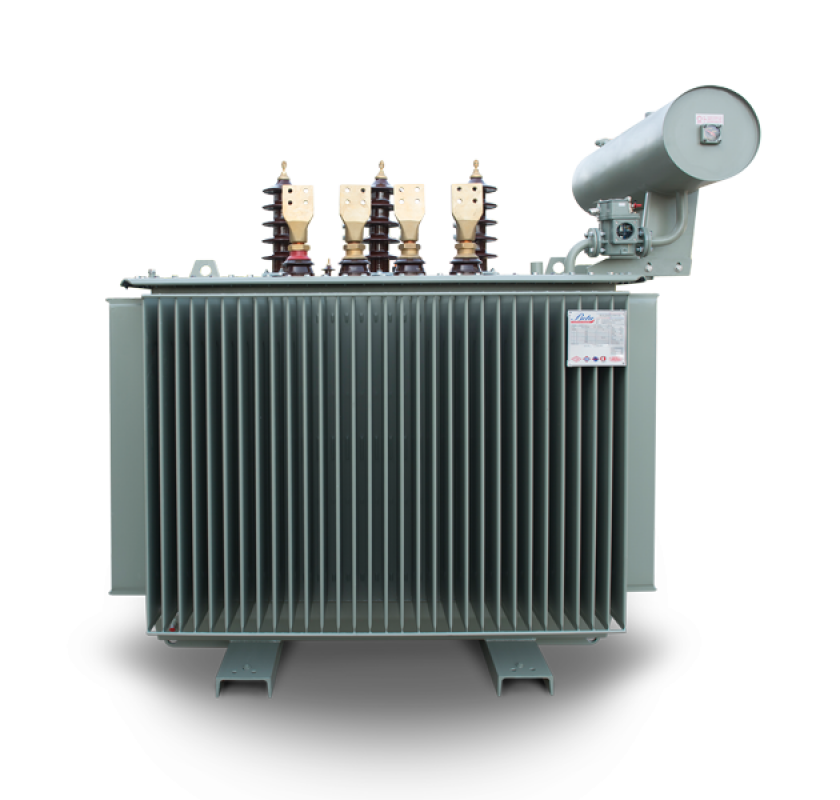
\includegraphics{../Figuras/Transformador}
    \par\end{center}


\end{frame}
\begin{frame}
  \frametitle{Motores}
  \begin{block} {Motor DC}
    \begin{itemize}
    \item $f_{1}=0$; $f_{L}=0$;\textrm{ $f_{2}=np$}
    \item Estator-Inductor alimentado por corriente DC (o imanes
      permanentes).
    \item El colector de delgas transforma la frecuencia de
      alimentación (DC) en alterna.
    \item Rotor-Inducido gira sincronizado con la frecuencia
      {}``transformada''.
    \end{itemize}
  \end{block}

\end{frame}
\begin{frame}
  \frametitle{Motores}
  \begin{block} {Motor asíncrono o de inducción}
    \begin{itemize}
    \item $f_{1}\neq0$; \textrm{$f_{L}=f_{2}=f_{1}-np$}
    \item Estator-inductor alimentado por una corriente trifásica
      alterna. Produce un campo giratorio.
    \item Rotor-inducido constituido por espiras cortocircuitadas
      (jaula de ardilla).
    \item Se produce un par que busca alinear el eje de las espiras
      con el campo inducido. El rotor se mueve siguiendo al campo
      giratorio.
    \item La velocidad de giro es inferior a la frecuencia de
      alimentación (asíncrono).
    \end{itemize}
  \end{block}
  Videos: Motor de inducción artesanal
  \href{http://www.youtube.com/watch?v=ZRGlAu0uCHY&feature=related}{(1)}
  \href{http://www.youtube.com/watch?v=P-eTLmJC2cQ}{(2)}
\end{frame}

\begin{frame}
  \frametitle{Generadores}
  \begin{block} {Generador Síncrono o Alternador}
    \begin{itemize}
    \item $f_{1}=0$; \textrm{$f_{L}=f_{2}=np$}
    \item Rotor-inductor alimentado por corriente continua mediante
      anillos.
    \item Estator-inducido constituido por un devanado trifásico.
    \item Al aplicar energía mecánica en el eje del rotor y
      alimentarlo con corriente continua, se obtiene una fuerza
      electromotriz en el estator.
    \item Empleado en turbinas hidráulicas y térmicas.
    \end{itemize}
  \end{block}

\end{frame}
\begin{frame}
  \frametitle{Generadores}
  \begin{block} {Dinamo}
    \begin{itemize}
    \item $f_{1}=0$; $f_{L}=0$;\textrm{ $f_{2}=np$}
    \item Estator-Inductor alimentado por corriente DC (o imanes
      permanentes).
    \item El colector de delgas transforma la frecuencia de
      alimentación (DC) en alterna.
    \item Al aplicar energía mecánica en el eje del rotor y alimentar
      el estator con corriente continua, se obtiene una fuerza
      electromotriz en el inducido con $f_{2}$.
    \item Las delgas rectifican para obtener $f_{L}=0$ en la salida.
    \end{itemize}
  \end{block}

\end{frame}
\section{Aparamenta eléctrica}


\begin{frame}
  \frametitle{Definición}


  \framesubtitle{ITC-BT-01}
  \begin{description}
  \item [{Aparamenta:}] Equipo, aparato o material previsto para ser
    conectado a un circuito eléctrico con el fin de asegurar una o
    varias de las siguientes funciones: protección, control,
    seccionamiento, conexión.
  \item [{Función~de~la~Aparamenta:}] Garantizar la seguridad de las
    personas, la continuidad en el suministro y la protección de los
    elemento de la instalación.
  \end{description}

\end{frame}
\begin{frame}[plain]
  \frametitle{Funciones de la aparamenta}
  \begin{itemize}
  \item \textbf{Protección}:

    \begin{itemize}
    \item Protección de los elementos de los circuitos contra las
      tensiones térmicas y mecánicas de las corrientes de
      cortocircuito.
    \item Protección de las personas en caso de producirse un defecto
      de aislamiento.
    \item Protección de los dispositivos y aparatos suministrados.
    \end{itemize}
  \item \textbf{Aislamiento}: separar de forma verificable un
    circuito, un aparato o un elemento de la planta del resto de un
    sistema que se encuentra en tensión, con el fin de que el personal
    pueda realizar con total seguridad trabajos en la parte aislada.
  \item \textbf{Control:} modificar un sistema cargado en cualquier
    momento

    \begin{itemize}
    \item Control funcional (conmutación rutinaria, etc.).
    \item Conmutación de emergencia.
    \item Operaciones de mantenimiento del sistema de alimentación.
    \end{itemize}
  \end{itemize}

\end{frame}
\begin{frame}
  \frametitle{Arco Eléctrico}
  \begin{description}
  \item [{Arco~eléctrico:}] descarga eléctrica que se forma entre dos
    electrodos sometidos a una diferencia de potencial. Durante el
    tiempo de la descarga se produce una luminosidad muy intensa y un
    gran desprendimiento de calor. Ambos fenómenos, en caso de ser
    accidentales, pueden ser sumamente destructivos.\end{description}
  \begin{block} {}
    \centering Video:
    \href{http://www.youtube.com/watch?v=WBTvGqRA4_0}{Apertura en Alta
      Tensión}
  \end{block}

\end{frame}
\begin{frame}
  \frametitle{Poder de corte y cierre}
  \begin{description}
  \item [{Poder~de~corte:}] intensidad de corriente que este
    dispositivo es capaz de cortar, bajo una tensión de
    restablecimiento determinada.
  \item [{Poder~de~cierre:}] intensidad de corriente que este aparato
    es capaz de establecer, bajo una tensión dada.
  \end{description}

\end{frame}
\begin{frame}
  \frametitle{Dispositivos simples}
  \begin{description}
  \item [{Seccionador:}] dispositivo de dos posiciones
    (abierto/cerrado) enclavable y accionado manualmente que
    proporciona un aislamiento seguro de un circuito cuando está
    enclavado en la posición abierta.  Un seccionador no está diseñado
    para abrir o cerrar el paso de la corriente.
  \item [{Interruptor~de~carga:}] dispositivo no automático
    (accionamiento manual) de dos posiciones (abierto/cerrado). Se
    utiliza para cerrar y abrir circuitos cargados en condiciones
    normales de circuitos sin defectos.
  \end{description}

\end{frame}
\begin{frame}
  \frametitle{Dispositivos simples}
  \begin{description}
  \item [{Contactor:}] dispositivo accionado por solenoide que por lo
    general se mantiene cerrado mediante una corriente (reducida) que
    pasa a través del solenoide de cierre. Se suelen controlar de
    forma remota por medio de pulsadores de activación/desactivación.
  \item [{Fusible:}] un filamento o lámina de un metal o aleación de
    bajo punto de fusión que se intercala en un punto determinado de
    una instalación eléctrica para que se funda, por Efecto Joule,
    cuando la intensidad de corriente supere, por un cortocircuito o
    un exceso de carga. Es capaz de abrir un circuito en carga.
  \end{description}

\end{frame}
\begin{frame}
  \frametitle{Interruptores automáticos}
  \begin{description}
  \item [{Interruptor~magnetotérmico:}] dispositivo capaz de
    interrumpir la corriente eléctrica de un circuito cuando ésta
    sobrepasa ciertos valores máximos. Su funcionamiento se basa en
    dos de los efectos producidos por la circulación de corriente
    eléctrica en un circuito: el magnético y el térmico (efecto
    Joule). El dispositivo consta, por tanto, de dos partes, un
    electroimán y una lámina bimetálica, conectadas en serie y por las
    que circula la corriente que va hacia la carga. Se emplea para
    \textbf{proteger contra sobreintensidades y sobrecargas}.
  \end{description}
  \begin{block}{}
    \centering Video:
    \href{http://www.youtube.com/watch?v=c6QqnLgWbCQ}{Apertura de un
      PIA}
  \end{block}

\end{frame}
\begin{frame}
  \frametitle{Interruptor Magnetotérmico}

  \begin{center}
    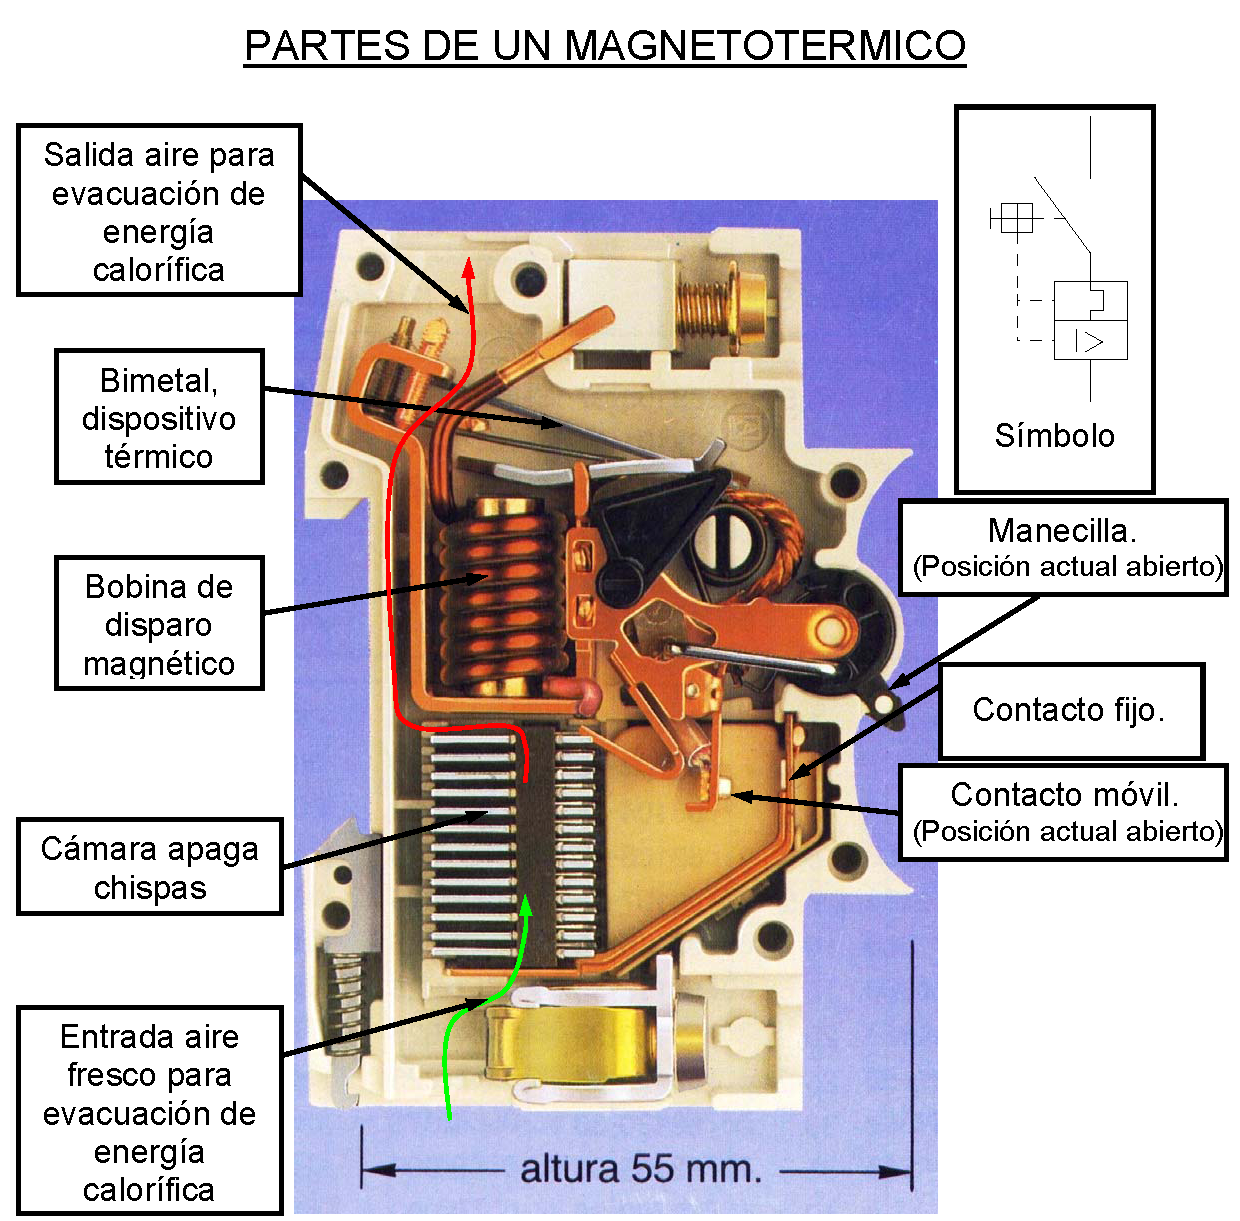
\includegraphics[scale=0.3]{../Figuras/Figuras_Externas/SeccionMagnetotermico}
    \par\end{center}


\end{frame}
\begin{frame}
  \frametitle{Interruptores automáticos}
  \begin{description}
  \item [{Interruptor~diferencial:}] dispositivo capaz de interrumpir
    la corriente eléctrica de un circuito cuando existe una corriente
    diferencial residual, indicativa de un defecto de
    aislamiento. Para la detección emplea un transformador toroidal
    que abraza a todos los conductores.  Cuando existe un defecto, la
    suma fasorial de las corrientes abarcadas no será nula y, por
    tanto, aparecerá una intensidad en el secundario del
    transformador, proporcional al defecto. Se emplea para la
    \textbf{protección de las personas}.
  \end{description}

\end{frame}
\begin{frame}
  \frametitle{Interruptor Diferencial}
  \begin{columns}[c]%{}


    \column{4cm}


    \begin{center}
      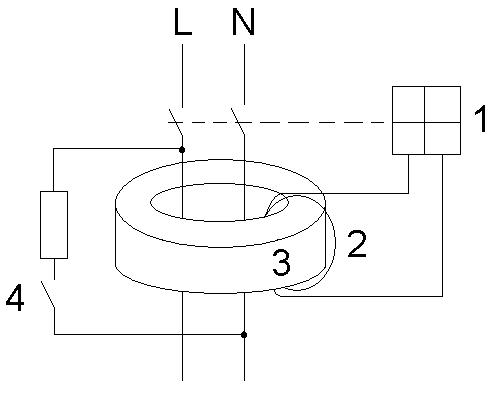
\includegraphics[scale=0.45]{../Figuras/Figuras_Externas/InterruptorDiferencial}
      \par\end{center}


    \column{4cm}


    \begin{center}
      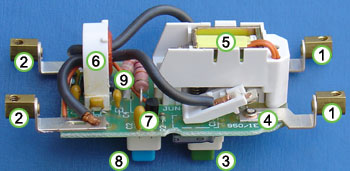
\includegraphics[scale=0.4]{../Figuras/Figuras_Externas/ResidualCurrentCircuitBreak}
      \par\end{center}

  \end{columns}%{}

\end{frame}


\section{Análisis en frecuencia}

\begin{frame}
  \frametitle{Análisis de Fourier}

  Un señal periódica puede ser descompuesta en sus armónicos mediante
  la serie de Fourier:
  \[
  x(t)=a_{0}+A_{1}\cdot\sin(\omega t+\phi_{1})+A_{2}\cdot\sin(2\omega
  t+\phi_{2})+...
  \]


  donde $A_{n}\cdot\sin(n\omega t+\phi_{n})$ es el armónico de orden n
  de la señal $x(t)$ y $a_{0}$es el valor medio de $x(t)$.

  Por ejemplo, una señal pura de 50 Hz, tendrá $a_{0}=0,$ y $A_{n}=0$
  salvo $A_{1}$.

  El armónico de primer orden se conoce como armónico fundamental.


\end{frame}
\begin{frame}
  \frametitle{Armónicos}

  \begin{center}
    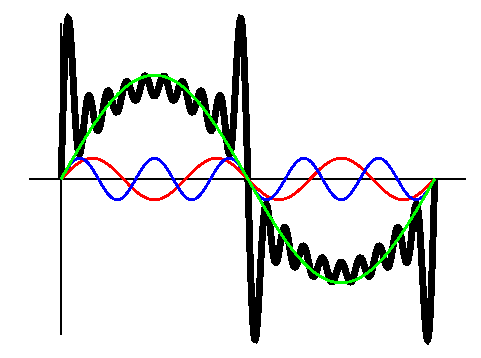
\includegraphics{../Figuras/Armonicos}
    \par\end{center}


\end{frame}
\begin{frame}[plain]
  \frametitle{Distorsión armónica}

  En general, los armónicos son inevitables pero indeseables. Para
  caracterizar el contenido en armónicos se utiliza:
  \begin{itemize}
  \item \textbf{Distorsión armónica total (THD)}: medida de la
    similitud entre la forma de la onda y su componente fundamental
    \[
    THD=\frac{1}{A_{1}}\cdot\sqrt{\sum_{n=2}^{\infty}A_{n}^{2}}
    \]

  \item \textbf{Factor de distorsión (FD)}: cociente entre el valor
    eficaz del armónico fundamental y el valor eficaz de la señal
    \[
    FD=\frac{A_{1}}{\sqrt{\sum_{n=0}^{\infty}A_{n}^{2}}}
    \]

\end{itemize}
Cuando $a_{0}=0$ (señal sin componente de continua)
\[
FD_{a_{0}=0}=\frac{1}{\sqrt{1+THD^{2}}}
\]



\end{frame}
\begin{frame}
  \frametitle{Potencia aparente}

  Al existir distorsión,
  \[
  S^{2}\neq P^{2}+Q^{2}
  \]


  Se define una nueva potencia, la potencia de distorsión
  \[
  D=\sqrt{S^{2}-P^{2}-Q^{2}}
  \]


  Por tanto, el factor de potencia
  \[
  FP=\frac{P}{S}\neq\cos(\phi_{1})
  \]


  Para señales sin componente continua, y suponiendo distorsión sólo
  en la onda de corriente:
  \[
  FP=FD\cdot\cos(\phi_{1})=\frac{\cos(\phi_{1})}{\sqrt{1+THD^{2}}}
  \]



\end{frame}


\section{Recursos}

\begin{frame}
  \frametitle{Bibliografía}
  \begin{itemize}
  \item \textbf{Fraile Mora, J.}: \emph{Electromagnetismo y circuitos
      eléctricos}. Ed. Mc. Graw Hill.
  \item \textbf{Fraile Mora, J.}: \emph{Máquinas
      Eléctricas}. Ed. Mc. Graw Hill.
  \item \textbf{Hayt, W. y Kemmerly, J}: \emph{Análisis de circuitos
      en ingeniería}. Ed. Mc. Graw Hill.
  \end{itemize}
\end{frame}

\begin{frame}
  \frametitle{Enlaces útiles}

  \begin{itemize}
  \item \href{http://www.directindustry.com/}{Equipos industriales}
  \item
    \href{http://www.schneiderelectric.es/sites/spain/es/productos-servicios/distribucion-electrica/descarga/pdf-guia-diseno-instalaciones-electricas.page}{Guía
      de diseño de instalaciones eléctricas (Schneider Electric)}
  \item \href{http://www.preoc.es/}{Base de Precios PREOC}
  \item \href{http://tuveras.com/index.html}{Tú verás}
  \item
    \href{http://www.f2i2.net/legislacionseguridadindustrial/legislacionNacionalGrupo.aspx?idregl=76}{Reglamento
      Electrotécnico de Baja Tensión}
  \end{itemize}

\end{frame}


\end{document}
